\documentclass[11pt]{exam}
\usepackage[utf8]{inputenc}
\usepackage{natbib}
\usepackage{hyperref}
\usepackage{graphicx}

\title{Evaluación del Módulo 5.2}
\author{Laura Rodríguez Navas \\ rodrigueznavas@posgrado.uimp.es}
\date{Marzo 2020}

\pagestyle{plain}

\begin{document}
	
\maketitle

\begin{questions}

% Pregunta 1
{\bf \question Defina la tarea de Recuperación de Información (2 puntos).}

La Recuperación de Información es la tarea que trata de satisfacer las necesidades de información de los usuarios, es decir, ante una consulta de un usuario, un sistema de recuperación de información busca en una colección de documentos aquel documento o fragmento de texto existente en una base de datos documental, que resuelve la consulta planteada por el usuario. 

Las necesidades de información de los usuarios, que se representan a través de consultas en lenguaje natural, se resuelven con los sistemas de RI, que seleccionan los documentos o textos que contienen estos términos de las consultas, para ayudar y permitir a los usuarios a acceder a gran cantidad de información textual disponible en Internet. 

El objetivo de los sistemas de RI es determinar si los términos seleccionados que contienen los documentos o textos son relevantes, y deben incorporar el concepto de normalización u orden de relevancia. 

Un sistema RI:

\begin{itemize}
	\item Se parte de una colección de documentos para representar otros documentos o fragmentos de texto y consultas (lenguaje de representación).
	\item Un usuario tiene una necesidad de información y plantea una consulta al sistema para procesar documentos (indexación) y consultas.
	\item Devuelve los documentos relevantes, que satisfacen la necesidad de información del usuario, seguramente normalizando los documentos para obtener una aproximación de la relevancia de estos en una consulta (cálculo de relevancia o similitud).
\end{itemize}

Los sistemas RI normalmente son evaluados en términos de la capacidad de recuperar exclusivamente documentos relevantes (efectividad) y en la complejidad y los tiempos de respuesta (eficiencia).

% Pregunta 2
{\bf \question Describa el modelo espacio vectorial en Recuperación de Información (2 puntos).}

El Modelo Espacio Vectorial es un modelo clásico de RI y es el modelo más utilizado por su eficiencia y facilidad de implementación, con un enfoque fundamentado matemáticamente.

\newpage

Características del modelo:

\begin{itemize}
	\item Representa los documentos como vectores de pesos de términos. \\
	Un documento es un vector de pesos \\
	\begin{center}
		$d = [w_{d,1}, ..., w_{d,i}, ..., w_{d,T}]$
	\end{center}
	donde cada peso es el producto la frecuencia de los términos(tf) y la frecuencia inversa de los documentos(idf)
		\begin{center}
		$w_{d,i} = tf_{d,i} * idf_{i}$
	\end{center}
	\item Utiliza técnicas de comparación de vectores: la medida de similitud coseno. \\
	Puede suceder que "vectores similares" tengan longitudes diferentes, así que los normalizamos, antes de compararlos para que tengan la misma longitud euclidiana.
	\item Se basa en álgebra vectorial.
	\item Permite el ajuste parcial y el ranking (necesidad de normalizar).
	\item Proporciona resultados ordenados.
	\item Permite la implementación eficiente para grandes colecciones de documentos.
\end{itemize}

% Pregunta 3
{\bf \question Defina las medidas de evaluación Precisión y Recall en el contexto de la Recuperación de Información (2 puntos).}

La precisión y recall son medidas de evaluación para evaluar los sistemas de RI.

La precisión es la ratio entre el número de documentos relevantes recuperados y el número de documentos recuperados. Es decir, la proporción entre documentos relevantes recuperados y documentos relevantes.

La recall se emplea en menor medida que la precisión y es la ratio de la proporción de documentos relevantes recuperados, comparado con el total de los documentos que son relevantes existentes en la base de datos, con total independencia de que éstos, se recuperen o no. Es decir, la proporción entre documentos relevantes recuperados y documentos recuperados.

Generalmente, la precisión y recall son medidas inversamente proporcionales y se suele buscar un equilibrio entre ellas o dar más importancia a la preferida por el usuario.

% Pregunta 4
{\bf \question ¿Qué es Lucene? ¿Y Solr? (2 puntos).}

\href{https://lucene.apache.org/core/}{Lucene} es una API de código abierto para recuperación de información, originalmente implementada en Java, que permite añadir funcionalidades de búsqueda a cualquier aplicación. 

Es una aplicación con mucha flexibilidad que le permite ser independiente del formato del fichero y trabajar con texto proveniente de una base de datos, de una página Web o de documentos en distintos formatos (.txt, .doc, .pdf, ...).

\newpage

Conceptos básicos:

\begin{itemize}
	\item Debe definirse la estructura de los documentos a buscar indicando los	campos que deben ser indexados o no.
	\item Debe definirse el análisis lingüístico (tokenización, stopper, stemmer, ...) que se le aplica a los documentos y a las consultas.
	\item Los documentos deben indexarse para hacer la búsqueda más eficiente.
	\item Debe definirse un lenguaje propio de consultas para recuperar los documentos.
	\item Debe realizarse la búsqueda sobre los índices y los documentos asociados a las consultas.
\end{itemize}

Lucene es útil para cualquier aplicación que requiera indexado y búsqueda a texto completo y se ha usado ampliamente por su utilidad en la implementación de motores de búsquedas.  

\href{https://lucene.apache.org/solr/}{Solr} es un sistema basado en Lucene que facilita el desarrollo de servidores de búsqueda. Proporciona indexación distribuida, replicación y consultas con equilibrio de carga, recuperación y conmutación por error automatizadas, configuración centralizada y más. También potencia las funciones de búsqueda y navegación de muchos de los sitios de Internet más grandes del mundo.

Lucene y Solr se han desarrollado por \href{http://www.apache.org/}{Apache Software Foundation}.

% Pregunta 5
{\bf \question Tras tres lecciones sobre Recuperación de Información, si le dijeran que tiene que diseñar un buscador de documentos ¿cuál sería la arquitectura de su sistema? No se limite al sistema de Recuperación de Información, piense que al menos necesita de una fuente de documentos, y que debe presentar los resultados de la búsqueda. (2 puntos).}

\subsection*{Arquitectura de Recuperación de la Información}

\begin{center}
	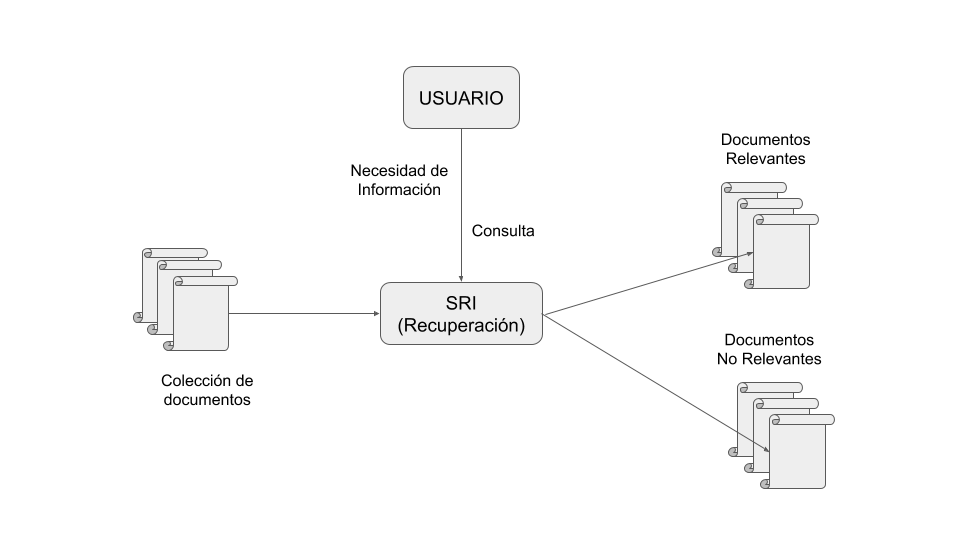
\includegraphics[scale=0.45]{general.png}
\end{center}

\subsection*{Arquitectura de mi sistema de RI}

\begin{center}
	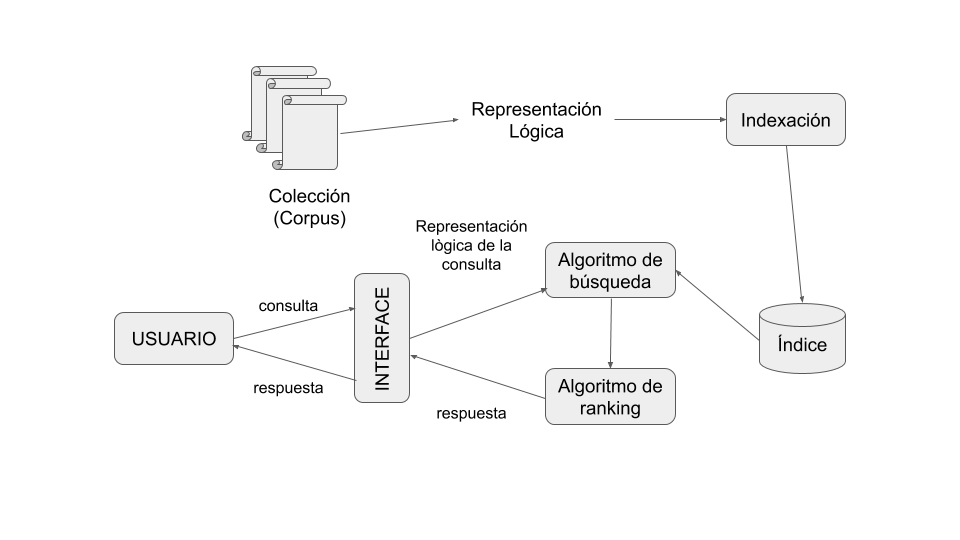
\includegraphics[scale=0.45]{sistema.png}
\end{center}

Componentes de la arquitectura de mi sistema RI:

\begin{itemize}
	\item La colección documentos de texto y corpus o base de datos textual. Para poder realizar operaciones sobre un corpus, es necesario primero una representación lógica de todos sus documentos, que puede consistir en un conjunto de términos, frases u otras unidades (sintácticas o semánticas) que permitan caracterizarlos.
	\item A partir de la representación lógica de los documentos, existe un proceso de indexación, que lleva a cabo la construcción de estructuras de datos (normalmente denominadas índices) que las almacene. Estas estructuras darán luego soporte a las búsquedas eficientes.
	\item El algoritmo de búsqueda acepta como entrada una expresión de consulta de un usuario y verifica en el índice cuales documentos pueden satisfacerlo. Luego, un algoritmo de ranking determina la relevancia de cada documento y retorna una lista con la respuesta. El primer ítem de dicha lista corresponde al documento más relevante y así sucesivamente en orden decreciente.
	\item La interfaz de usuario permite que este especifique la consulta mediante una expresión escrita en un lenguaje preestablecido y sirve para mostrar las respuestas retornadas por el sistema.
\end{itemize}

\end{questions}
	
\end{document}
